\documentclass[11pt,a4paper]{article}
\usepackage[T1]{fontenc}
\usepackage[utf8]{inputenc}
\usepackage[spanish,es-noshorthands]{babel}
\usepackage[margin=2.5cm]{geometry}
\usepackage{enumitem}
\usepackage{url}
\usepackage{graphicx}
\graphicspath{{figs/}}
\setlist{itemsep=2pt}

\title{Menú 3: calibración del Citiroc con los pulsos oscuros}
\author{JJ}
\date{\today}

\begin{document}
\maketitle

\section*{Aperitivo}

\begin{enumerate}
\item Tarjeta CAEN A5202 (dos Citiroc~1A, 64 canales), leída a través del
  concentrador DT5215 con el programa de adquisición de datos (DAQ) de JMB.
\item Los nombres de los parámetros son los del DAQ de JMB, que coinciden con
  los del software de CAEN (Janus, Sección~\ref{sec:janus}).
\item \sloppy El chip trabaja en modo peak stretch. En Janus es
  \texttt{PeakDetectorMode} = PEAK\_STRETCH; en el DAQ de JMB es el modo por
  defecto y no hay que configurar nada.
  La
  cadena del Citiroc, el peak stretch y la ventana se explican en el
  menú~1, Sección~1.
\end{enumerate}

\section{Qué mide la calibración}
\label{sec:medida}

\begin{figure}[!ht]
\centering
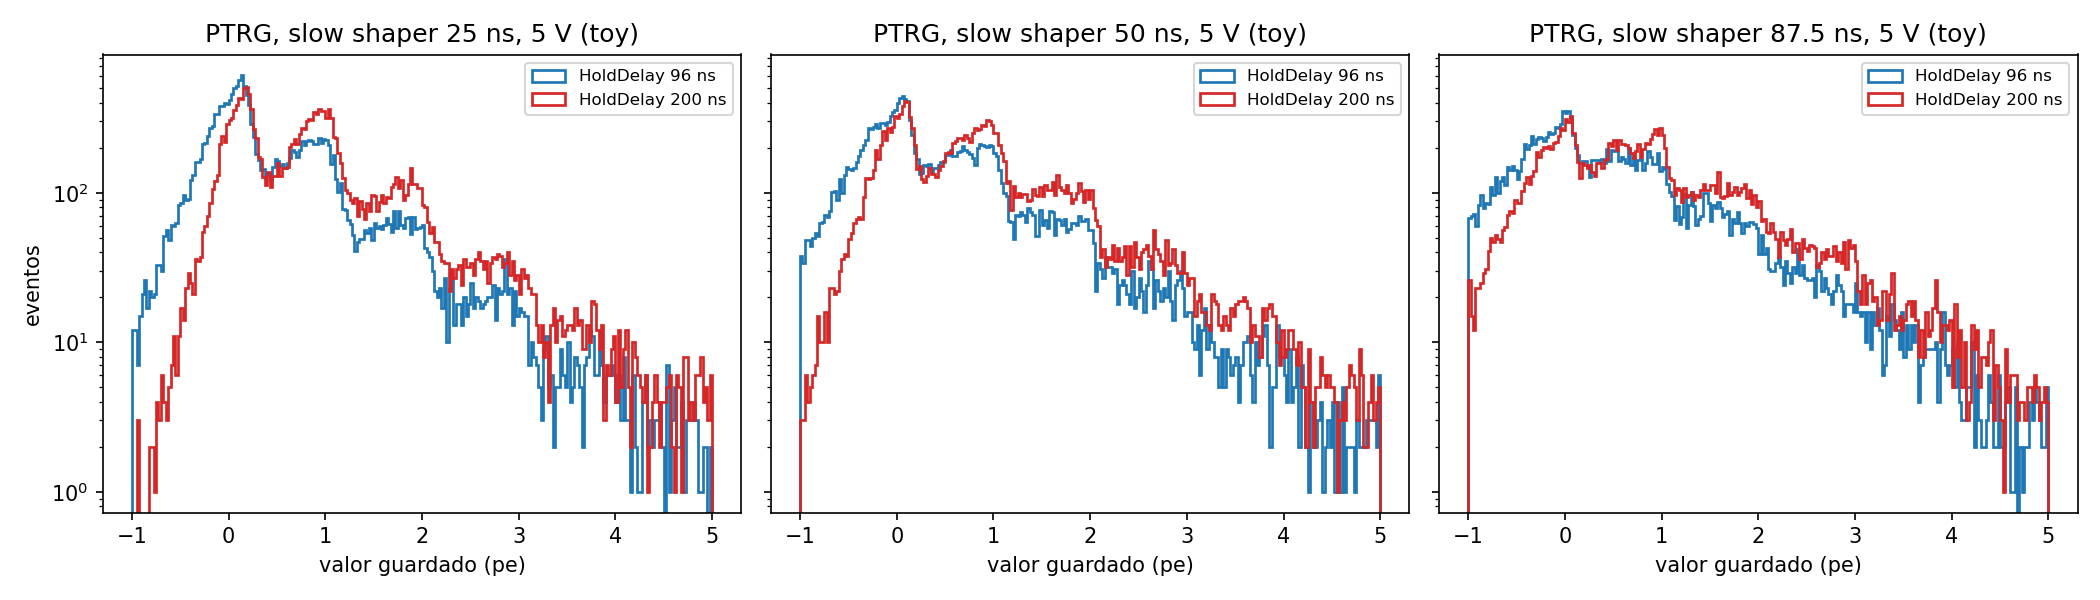
\includegraphics[width=\textwidth]{spe_ptrg.png}
\caption{Espectro de alta ganancia de un canal con trigger periódico, a
5~V, según un modelo sencillo con DP a 4,4~MHz, crosstalk del 19,5\,\% y
ruido, para slow shaper de 25, 50 y 87,5~ns y \texttt{HoldDelay} de 96 y
200~ns. Los picos de 0, 1, 2 y 3~pe tienen el borde derecho afilado, en la
altura de cada pe, y una cola hacia la izquierda de los pulsos que la
ventana corta. A 25~ns la escalera es la más limpia; a 87,5~ns los DP se
apilan y la emborronan.}
\label{fig:ptrg}
\end{figure}

\subsection*{La ganancia con los pulsos oscuros}

\begin{itemize}
\item Por encima de la tensión de ruptura (breakdown voltage, BV) cada
  canal da pulsos oscuros (dark pulses, DP), varios MHz por canal. Casi
  todos son de un fotoelectrón (pe); los que encienden otras celdas por
  crosstalk son de 2, 3\ldots~pe. Su espectro es una escalera de picos
  igualmente espaciados: la distancia entre picos es la ganancia del canal,
  en cuentas de ADC por pe. Es la unidad de toda la cadena: la simulación
  expresa cada carga en pe.
\item La calibración se hace en la alta ganancia, con un shaping corto, que
  separa los picos (menú~1, Sección~1). La ganancia se pasa luego a la baja
  ganancia, la de la energía, con el cociente medido entre las dos.
\end{itemize}

\subsection*{Con trigger periódico}



\begin{itemize}
\item Con el trigger periódico (PTRG) la ventana cae en un instante
  cualquiera, sin relación con los DP. En peak stretch el chip guarda el
  máximo de la salida del slow shaper (SS) en esa ventana, que dura el
  \texttt{HoldDelay}. Si ningún DP llega a su máximo dentro de la ventana,
  el valor es el pedestal; si llega uno de 1~pe, 1~pe; y así sucesivamente
  (Figura~\ref{fig:ptrg}).
\item Así se calibran los 64 canales a la vez, en todos los eventos, sin
  depender del umbral del discriminador, del fast shaper ni de la latencia
  de la tarjeta: el trigger no sale de los DP.
\item La ventana decide cuántos eventos caen en cada pico: con 200~ns, en
  unos dos de cada tres eventos llega algún DP. Un DP que tiene su máximo
  fuera de la ventana pero parte del pulso dentro deja un valor menor que
  su altura: es la cola a la izquierda de cada pico. Por eso la posición de
  cada pico es la de su máximo, cerca del borde derecho, y no el centro de
  una gaussiana; el mismo criterio se aplica al espectro simulado.
\item Con el \texttt{HoldDelay} = 200~ns de esta nota, a 25~ns los picos
  de 1, 2 y 3~pe se separan bien; a 87,5~ns se emborronan. La
  Figura~\ref{fig:ptrg} muestra los dos efectos.
\end{itemize}

\subsection*{El cero de la escalera}

\begin{itemize}
\item La recta que pasa por los picos de 1, 2 y 3~pe da la ganancia
  (pendiente) y el cero de la escalera (ordenada en el origen). En el
  Citiroc el cero coincide con el pedestal medido por debajo del BV con el
  mismo shaping y \texttt{HoldDelay} (menú~1), salvo el pequeño
  desplazamiento que da el máximo del ruido en la ventana. Lo que se mueve
  es el pico de 0~pe: en los eventos sin DP el chip guarda el máximo de las
  colas negativas de los DP anteriores, y por eso se ensancha hacia abajo
  (Figura~\ref{fig:ptrg}). Comparar el cero con el pedestal comprueba la
  calibración.
\end{itemize}

\subsection*{Tensión y crosstalk}

\begin{figure}[!ht]
\centering
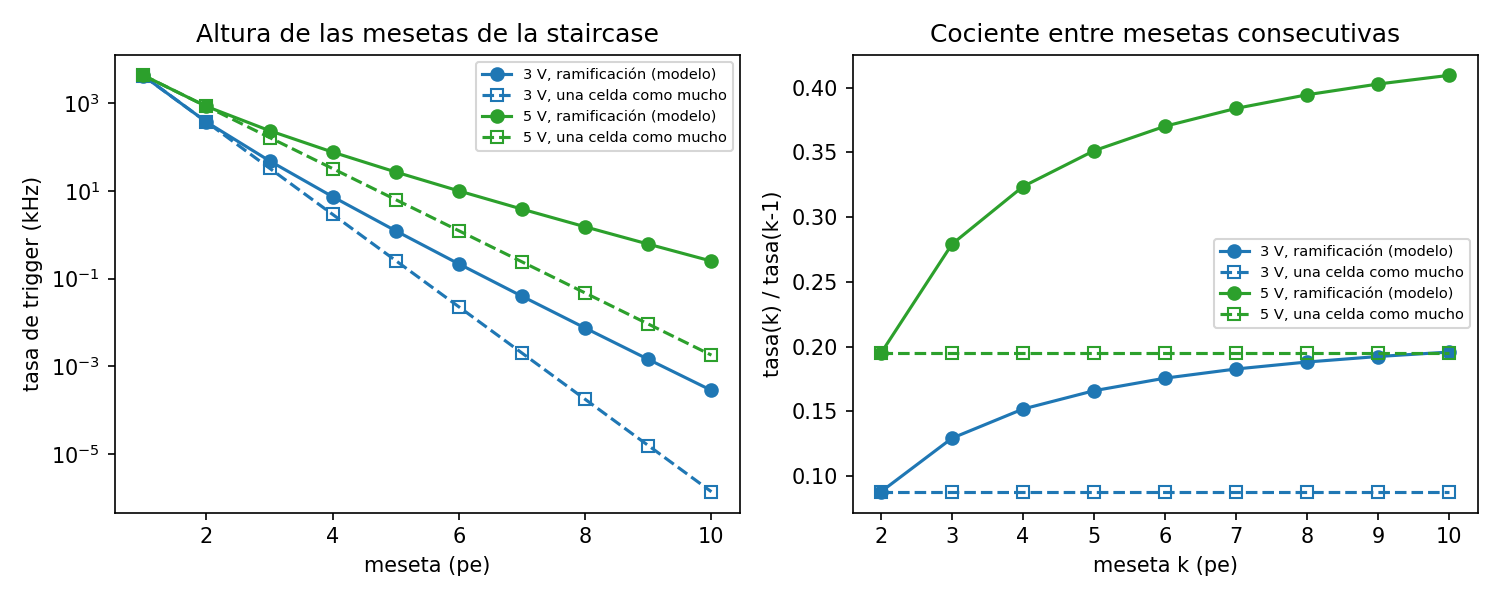
\includegraphics[width=\textwidth]{staircase_crosstalk.png}
\caption{Staircase hasta 10~pe según el modelo, a 3 y 5~V. Izquierda:
altura de las mesetas. Derecha: cociente entre mesetas consecutivas. Si
cada celda dispara como mucho a otra (cuadrados), el cociente es constante
e igual a la probabilidad de crosstalk. Con ramificación (círculos, el
modelo), crece con el número de pe: a 5~V, 0,20, 0,28, 0,32, 0,35\ldots}
\label{fig:crosstalk}
\end{figure}

\begin{itemize}
\item La ganancia es proporcional al overvoltage (la tensión por encima del
  BV). Con la ganancia a 3, 4 y 5~V, la recta frente a la tensión del canal
  corta el cero en su BV.
\item La staircase (menú~2, Sección~1) llevada hasta unos 10~pe da la tasa
  de DP con al menos 1, 2, 3\ldots~pe. El cociente entre mesetas
  consecutivas dice cómo es el crosstalk: constante si cada celda dispara
  como mucho a otra, creciente si se ramifica, como supone el modelo
  (Figura~\ref{fig:crosstalk}).
\end{itemize}

\section*{Programa de festejos}

\noindent {\bf Setup}
\begin{itemize}
\item {\bf Acción:}
  \begin{itemize}
  \item Montar sin cristal, con los SiPM conectados y a oscuras.
  \item Partir de la configuración de producción y cambiar en la pestaña
    {\bf Acquisition} solo los parámetros de la Sección~\ref{sec:janus}.
  \item \texttt{HV\_Vbias} para 5~V de overvoltage: unos 43~V a temperatura
    ambiente. Fijarlo antes de lanzar el run, no durante.
  \item Lanzar un run corto (nota 0) para que la tarjeta reciba la
    configuración y la tensión.
  \item En la pestaña {\bf Hardware}, encender el HV de la tarjeta y esperar
    a que Vmon e Imon estén estables.
  \end{itemize}
\item {\bf Resultado:} cada run se para solo a los 50\,000 eventos (50~s).
  El DAQ le asigna un número \texttt{N} y escribe \texttt{run\_N.0000.h5} y
  \texttt{run\_N.histograms.h5}, como en el menú~1.
\item {\bf Precaución:} al acabar el primer run, mirar en la pestaña
  {\bf Plots} el espectro de alta ganancia de algunos canales: deben verse
  los picos de 0, 1 y 2~pe. Si no se separan, parar y avisar antes de
  cambiar \texttt{HG\_Gain}.
\end{itemize}

\noindent {\bf Paso 1: SPE a 5~V con slow shaper de 25~ns}
\begin{itemize}
\item {\bf Acción:}
  \begin{itemize}
  \item \texttt{HG\_ShapingTime} = 25~ns.
  \item Un run.
  \end{itemize}
\item {\bf Resultado:} 1 run con sus dos ficheros.
\item {\bf Análisis:} el de la Sección~\ref{sec:datos}: la ganancia y el
  cero de cada canal. Es la calibración principal.
\end{itemize}

\noindent {\bf Paso 2: SPE a 5~V con slow shaper de 50 y 87,5~ns}
\begin{itemize}
\item {\bf Acción:}
  \begin{itemize}
  \item Un run con \texttt{HG\_ShapingTime} = 50~ns.
  \item Un run con \texttt{HG\_ShapingTime} = 87,5~ns.
  \end{itemize}
\item {\bf Resultado:} 2 runs, cada uno con sus dos ficheros.
\item {\bf Análisis:} la ganancia de cada canal con cada shaping, y si los
  picos se separan.
\end{itemize}

\noindent {\bf Paso 3: SPE a 4 y 3~V con slow shaper de 25~ns}
\begin{itemize}
\item {\bf Acción:}
  \begin{itemize}
  \item \texttt{HG\_ShapingTime} = 25~ns.
  \item \texttt{HV\_Vbias} 1~V menos (4~V de overvoltage), un run corto
    (nota 0), esperar a que Vmon e Imon estén estables, un run.
  \item \texttt{HV\_Vbias} otro voltio menos (3~V), un run corto, esperar,
    un run.
  \end{itemize}
\item {\bf Resultado:} 2 runs, cada uno con sus dos ficheros.
\item {\bf Análisis:} la ganancia de cada canal a 3, 4 y 5~V, y su BV.
\end{itemize}

\noindent {\bf Paso 4: staircase hasta 10~pe}
\begin{itemize}
\item {\bf Acción:}
  \begin{itemize}
  \item A 5~V, en la pestaña {\bf Scans}, Staircase, con el rango ampliado
    hasta unos 10~pe (Sección~\ref{sec:janus}) y \texttt{Dwell} = 500~ms.
  \item Lo mismo a 3~V, hasta unos 6~pe, con un run corto antes para
    aplicar la tensión.
  \end{itemize}
\item {\bf Resultado:} 2 staircases, cada una guardada como un run.
\item {\bf Análisis:} la altura de cada meseta y el cociente entre mesetas
  consecutivas.
\end{itemize}

\section*{Qué necesita el cocinero}

\begin{itemize}
\item De cada run, los dos ficheros \texttt{.h5}, y las dos staircases.
\item Una fila por run y por staircase en el logbook de la hoja de Google
  (nota 0), con la tensión y el shaping.
\item Si algo no se comporta como espera el menú, para y grita.
\end{itemize}

\section{Cómo entra la medida en el modelo}
\label{sec:razon}

\begin{itemize}
\item {\bf Ganancia.} El modelo da $0{,}93\times10^6$ electrones por voltio
  de overvoltage. La calibración simulada recupera la ganancia de cada
  canal con una dispersión de unos pocos por ciento a 25~ns, y peor con
  shaping más largo, porque los DP se apilan.
\item {\bf Cero.} El cero de la escalera debe coincidir con el pedestal
  del menú~1, con el mismo shaping y \texttt{HoldDelay}. La forma del pico
  de 0~pe, con su cola hacia abajo, depende de la tasa de DP y de la forma
  del pulso, y se compara con la simulación.
\item {\bf BV.} Fija el overvoltage de cada canal y, con su coeficiente de
  temperatura (34~mV por grado), la temperatura de los SiPM. El modelo
  toma 38,0~V a 25~$^\circ$C, con una dispersión de 0,1 a 0,2~V entre
  canales.
\item {\bf Crosstalk.} El modelo lo trata como una ramificación: cada celda
  que se dispara puede disparar a su vez a sus vecinas. Eso fija cuántos DP
  grandes hay y, con ellos, la tasa de triggers falsos en las medidas de
  energía. La staircase hasta 10~pe distingue los dos casos.
\item {\bf Tensión.} A 5~V la ganancia es 1,67 veces la de 3~V, pero hay
  más crosstalk (19,5\,\% frente a 8,8\,\%). Los runs a 3, 4 y 5~V dicen
  cuál de los dos efectos domina.
\end{itemize}

\section{Parámetros del DAQ (A5202)}
\label{sec:janus}

\begin{center}
\small
\begin{tabular}{p{0.3\textwidth} p{0.6\textwidth}}
\hline
parámetro & valor \\
\hline
\texttt{HV\_Vbias} & 5, 4 o 3~V por encima del BV, según el paso: unos 43,
42 o 41~V a temperatura ambiente \\
\texttt{HV\_IndivAdj} & 0 (como en producción) \\
\texttt{AcquisitionMode} & SPECTROSCOPY \\
\texttt{BunchTrgSource} & PTRG (trigger periódico, independiente de la señal) \\
\texttt{PtrgPeriod} & 1~ms: 50\,000 eventos en 50~s \\
\texttt{HoldDelay} & 200~ns \\
\texttt{HG\_ShapingTime} & 25, 50 o 87,5~ns, según el paso \\
\texttt{LG\_ShapingTime} & 87,5~ns \\
\texttt{HG\_Gain}, \texttt{LG\_Gain} & 55 (como en producción) \\
\texttt{GainSelect} & BOTH \\
\texttt{ZS\_Threshold\_HG}, \texttt{ZS\_Threshold\_LG} & 0, también en los
umbrales por canal si la configuración los tiene \\
\texttt{ChEnableMask0}, \texttt{ChEnableMask1} & todos los canales
({\bf Configure channels}, {\bf Enable all}) \\
\texttt{EnableServiceEvents} & activado \\
\texttt{StopRunMode}, \texttt{PresetCounts} & PRESET\_COUNTS, 50000 \\
{\bf Store run histograms} & activado \\
\hline
\end{tabular}
\end{center}

\noindent Los parámetros con índice del fichero de producción (por ejemplo
\texttt{TD\_CoarseThreshold[0]} o \texttt{ChEnableMask0[1]}) son de cada
tarjeta y mandan sobre el valor común: cambiarlos también, o quitarlos
(nota 0).

\noindent {\bf Rango de la staircase del paso 4.} La staircase del menú~2,
a 5~V, da la distancia entre los escalones de 1 y 2~pe en unidades de
\texttt{TD\_CoarseThreshold}: es 1~pe. \texttt{Maximum} se pone unos 9 de
esas distancias por encima del escalón de 1~pe (10~pe), y \texttt{Minimum}
justo por debajo de la meseta de 1~pe. A 3~V el pe es más pequeño: primero
una staircase como la del menú~2 para medir la distancia, y luego
\texttt{Maximum} unos 5 pasos por encima (6~pe). A 5~V la meseta de 10~pe
está en unos 250~Hz, así que 500~ms por punto dan más de 100 cuentas.

\section{Análisis}
\label{sec:datos}

\begin{itemize}
\item \sloppy {\bf Espectros.} Los datos están en
  \path{/events/spectroscopy/observations} de cada \texttt{run\_N.0000.h5}:
  para cada canal, el espectro de alta ganancia con los 50\,000 eventos, a
  resolución completa.
\item {\bf Ganancia y cero.} La posición de cada pico es la de su máximo
  (Sección~\ref{sec:medida}); la recta que pasa por los picos de 1, 2 y
  3~pe da la ganancia (pendiente, en cuentas de ADC por pe) y el cero
  (ordenada en el origen). El cero se compara con el pedestal del menú~1.
\item {\bf BV.} Para cada canal, la recta de la ganancia frente a
  \texttt{HV\_Vbias} con los puntos de 3, 4 y 5~V; su corte con el cero es
  el BV.
\item {\bf Crosstalk.} Para cada canal, la tasa de cada meseta de la
  staircase. La primera es la tasa de DP; el cociente de la segunda a la
  primera, la probabilidad de crosstalk; los siguientes cocientes, si el
  crosstalk se ramifica.
\end{itemize}

\section{Lo que se espera, según el modelo}

\begin{itemize}
\item {\bf Ganancia:} $4{,}6\times10^6$ electrones (0,75~pC) por pe a 5~V,
  $3{,}7\times10^6$ a 4~V y $2{,}8\times10^6$ a 3~V; en cuentas de ADC
  depende de \texttt{HG\_Gain}.
\item {\bf Espectros:} los de la Figura~\ref{fig:ptrg}: escalera limpia a
  25~ns, emborronada a 87,5~ns.
\item {\bf Cero:} igual al pedestal del menú~1, con el mismo shaping y
  \texttt{HoldDelay}.
\item {\bf BV:} 38,0~V a 25~$^\circ$C, y 34~mV menos por cada grado por
  debajo, con una dispersión de 0,1 a 0,2~V entre canales.
\item {\bf Staircase hasta 10~pe:} meseta de 1~pe a 4,4~MHz a 5~V y
  4,3~MHz a 3~V; cocientes, con ramificación, 0,20, 0,28, 0,32 y 0,35 a
  5~V, y 0,09, 0,13, 0,15 y 0,17 a 3~V.
\end{itemize}

\end{document}
